\section{Simulation Analysis}
\label{section:sim}
 
In this section, the several steps taken using ngspice in order to conduct the simulation of the audio amplifier, as requested, will be described. The main focus of the simulation was to determine and optimize de values of the gain, the cut off frequencies, both lower and upper and the bandiwidth. The quality and overall figure of merit will then be analysed.
The group proceded as follows:

\begin{enumerate}
\item Design of the circuit, having as a starting point the circuit given by the professor.

\item Verification of the operation of the transistors in the forward Active region, the called F.A.R mode. The results are shown below.

\begin{table}[ht]
  \centering
  \begin{tabular}{|l|r|}
    \hline    
   Vce & 1.57786\\ \hline
Vbe & 0.682323\\ \hline
Vce greater than Vbe & Correct F.A.R\\ \hline

     \end{tabular}
  \caption{Verification of the F.A.R mode in the NPN transistor}
 
\end{table}


\begin{table}[ht]
  \centering
  \begin{tabular}{|l|r|}
    \hline    
   Vec & 2.72908\\ \hline
Veb & 0.781397\\ \hline
Vec greater than Veb & Correct F.A.R\\ \hline

     \end{tabular}
  \caption{Verification of the F.A.R mode in the NPN transistor}
    
\end{table}



\item OP Analysis
     Then, the OP values of the currents and nodal voltages were computed. These are key to calculate the incremental parameters.
     
 \begin{table}[ht]

  \centering
  \begin{tabular}{|l|r|}
    \hline    
    {\bf Name} & {\bf Value [V,A]} \\ \hline
    @c1[i] & 0.000000e+00\\ \hline
@gb[i] & -2.26065e-04\\ \hline
@r1[i] & 2.161572e-04\\ \hline
@r2[i] & -2.26065e-04\\ \hline
@r3[i] & -9.90741e-06\\ \hline
@r4[i] & 1.183330e-03\\ \hline
@r5[i] & -2.26065e-04\\ \hline
@r6[i] & -9.67173e-04\\ \hline
@r7[i] & 9.671730e-04\\ \hline
v(1) & 5.068716e+00\\ \hline
v(2) & 4.843672e+00\\ \hline
v(3) & 4.369060e+00\\ \hline
v(5) & 4.874693e+00\\ \hline
v(6) & 5.579017e+00\\ \hline
v(7) & -1.98076e+00\\ \hline
v(8) & -2.97458e+00\\ \hline
v(9) & -1.98076e+00\\ \hline

  \end{tabular}
  \caption{Simulation nodal voltage results. All variables are expressed in V or A.} 
\end{table}
     
     
  
\item  In the frequency domain, measure of the output voltage gain, using the function .meas as well as the lower and upper cut off frequencies and the bandwidth.


\begin{table}[ht]
  \centering
  \begin{tabular}{|l|r|}
    \hline    
   Gain& 34.0105\\ \hline
Central Frequency& 794.328\\ \hline
Gain deviation&49.8206\\ \hline
Central frequency deviation&205.672\\ \hline

    \end{tabular}
  \caption{Results for ngspice}
    \label{tab:results}
\end{table}


The quantities obtained are desribed in the table \ref{tab:results}. The results obtained allowed the group to understand the functions of the different components of the circuit. 
The conclusions will be outlined.


 \textbf{EFFECT OF THE COUPLING CAPACITORS}

The coupling capacitors' main porpuse is to block the DC signals. If studying an incremental model of an audio amplifier, all values that are constant must be eliminated so the transistors are always fowardly conducting. As so, two coupling capacitors were used. Once the capacitors may also block some low frequencies, they have a direct influence in the bandwidth.


 \textbf{EFFECT OF THE BYPASS CAPACITOR}
 
  As studied in the lectures, the resistor Re has the funciton of stabelizing the effect of the temperature in the DC voltage. However, it has also a negative effect on the gain, once it lowers it. In order to solve the problem, a bypass capacitor Ce is placed in parallel with the resistor, so that the capacitor bypasses the resistor. In DC mode, the resistor plays its effect in the temperature. In AC, the resistor will not affect the gain. To sum up, the capacitor is a short-circuit for higher frequencies (AC) and a open-circuit for low frequencies (DC).


 \textbf{EFFECT OF RC}
 
IC is the most important current in the circuit because it determines gm, and so directly influences the gain, by increasing it.

\textbf{GRAPHICAL REPRESENTATION}

In the graphics \ref{sim4} and \ref{sim5}, a graphic representation of the effect pf the components above mentioned can be observed. In fact, in the plot \ref{sim5} is extremely enligtenment as one can intuitevely notice the high bandwidth, the stabilization of the gain, and the gain itself.


\begin{figure}[h] \centering
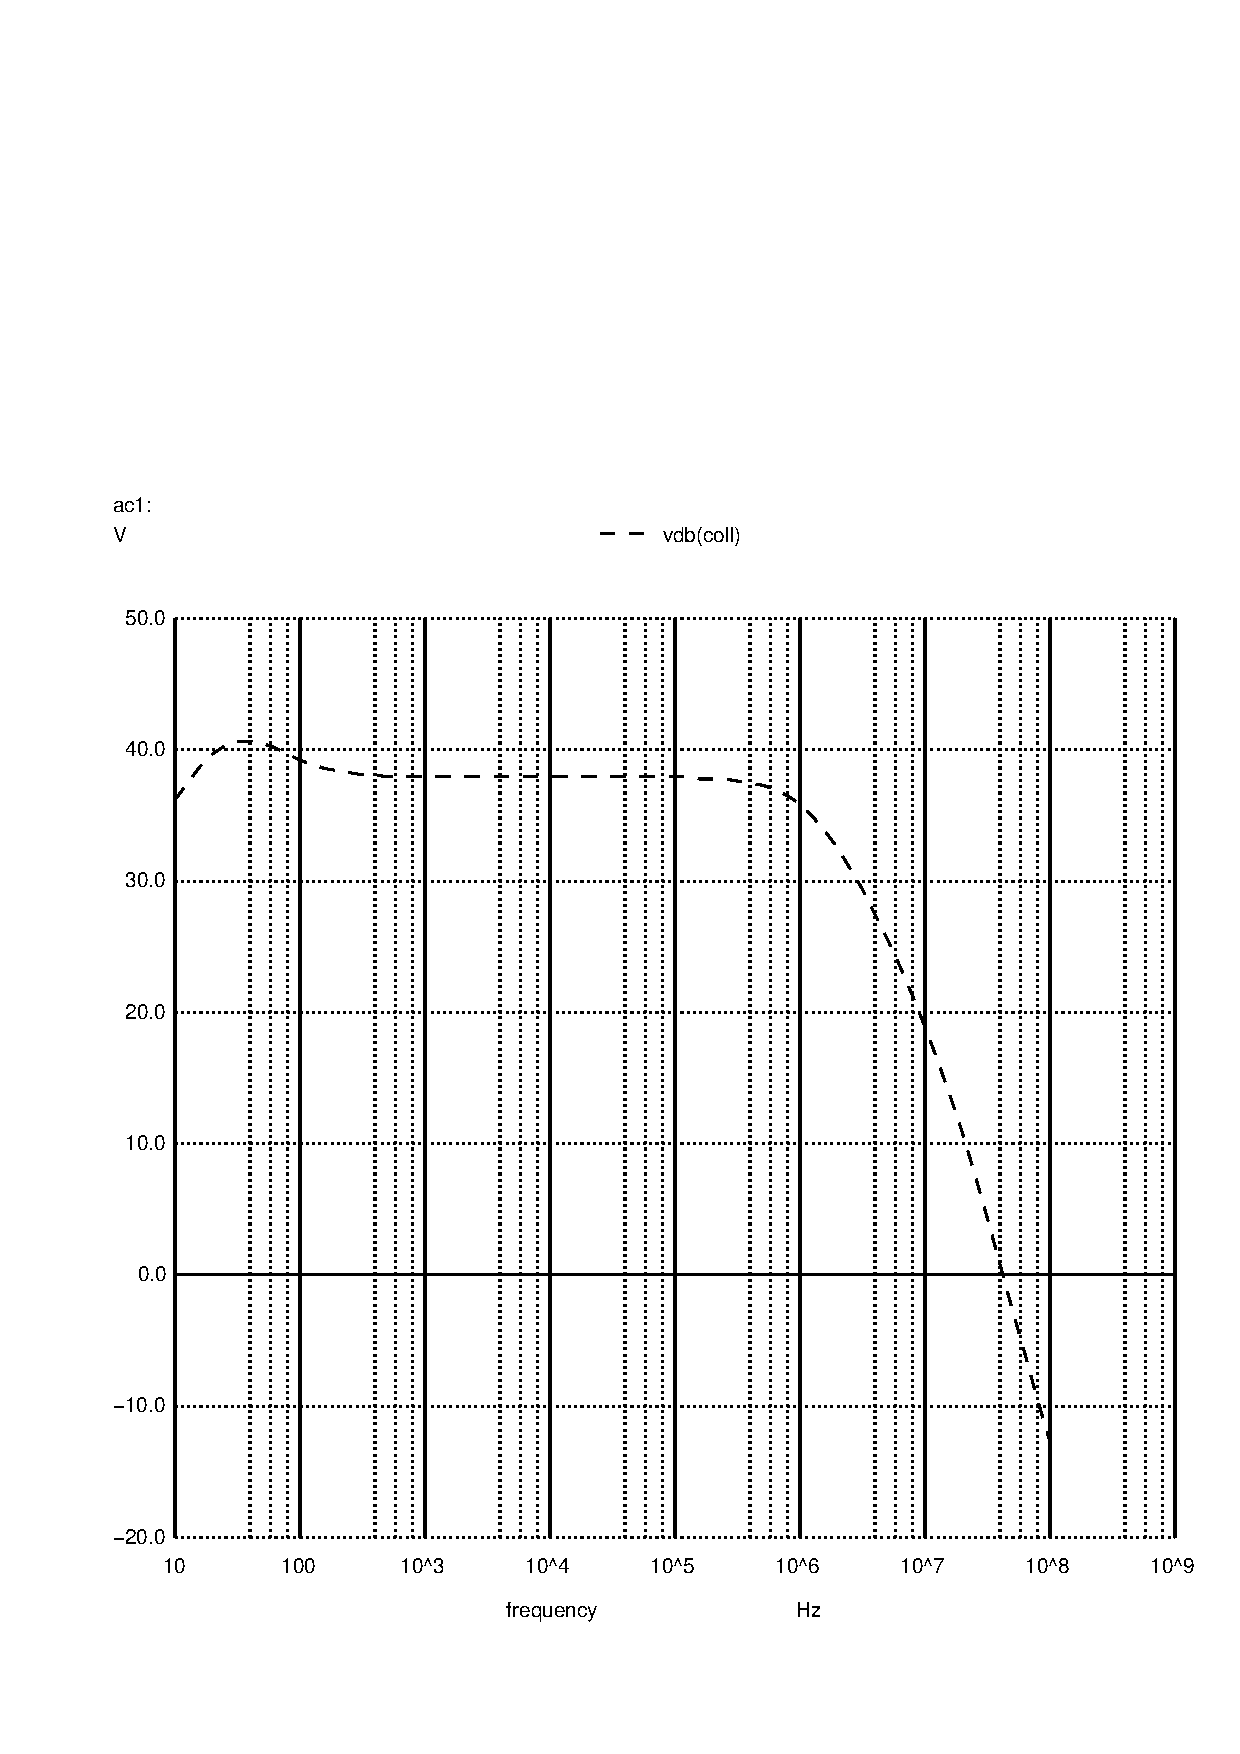
\includegraphics[width=0.4\linewidth]{vo1f.pdf}
\caption{Input Voltage}
\label{fig:sim4}
\end{figure}


\begin{figure}[h] \centering
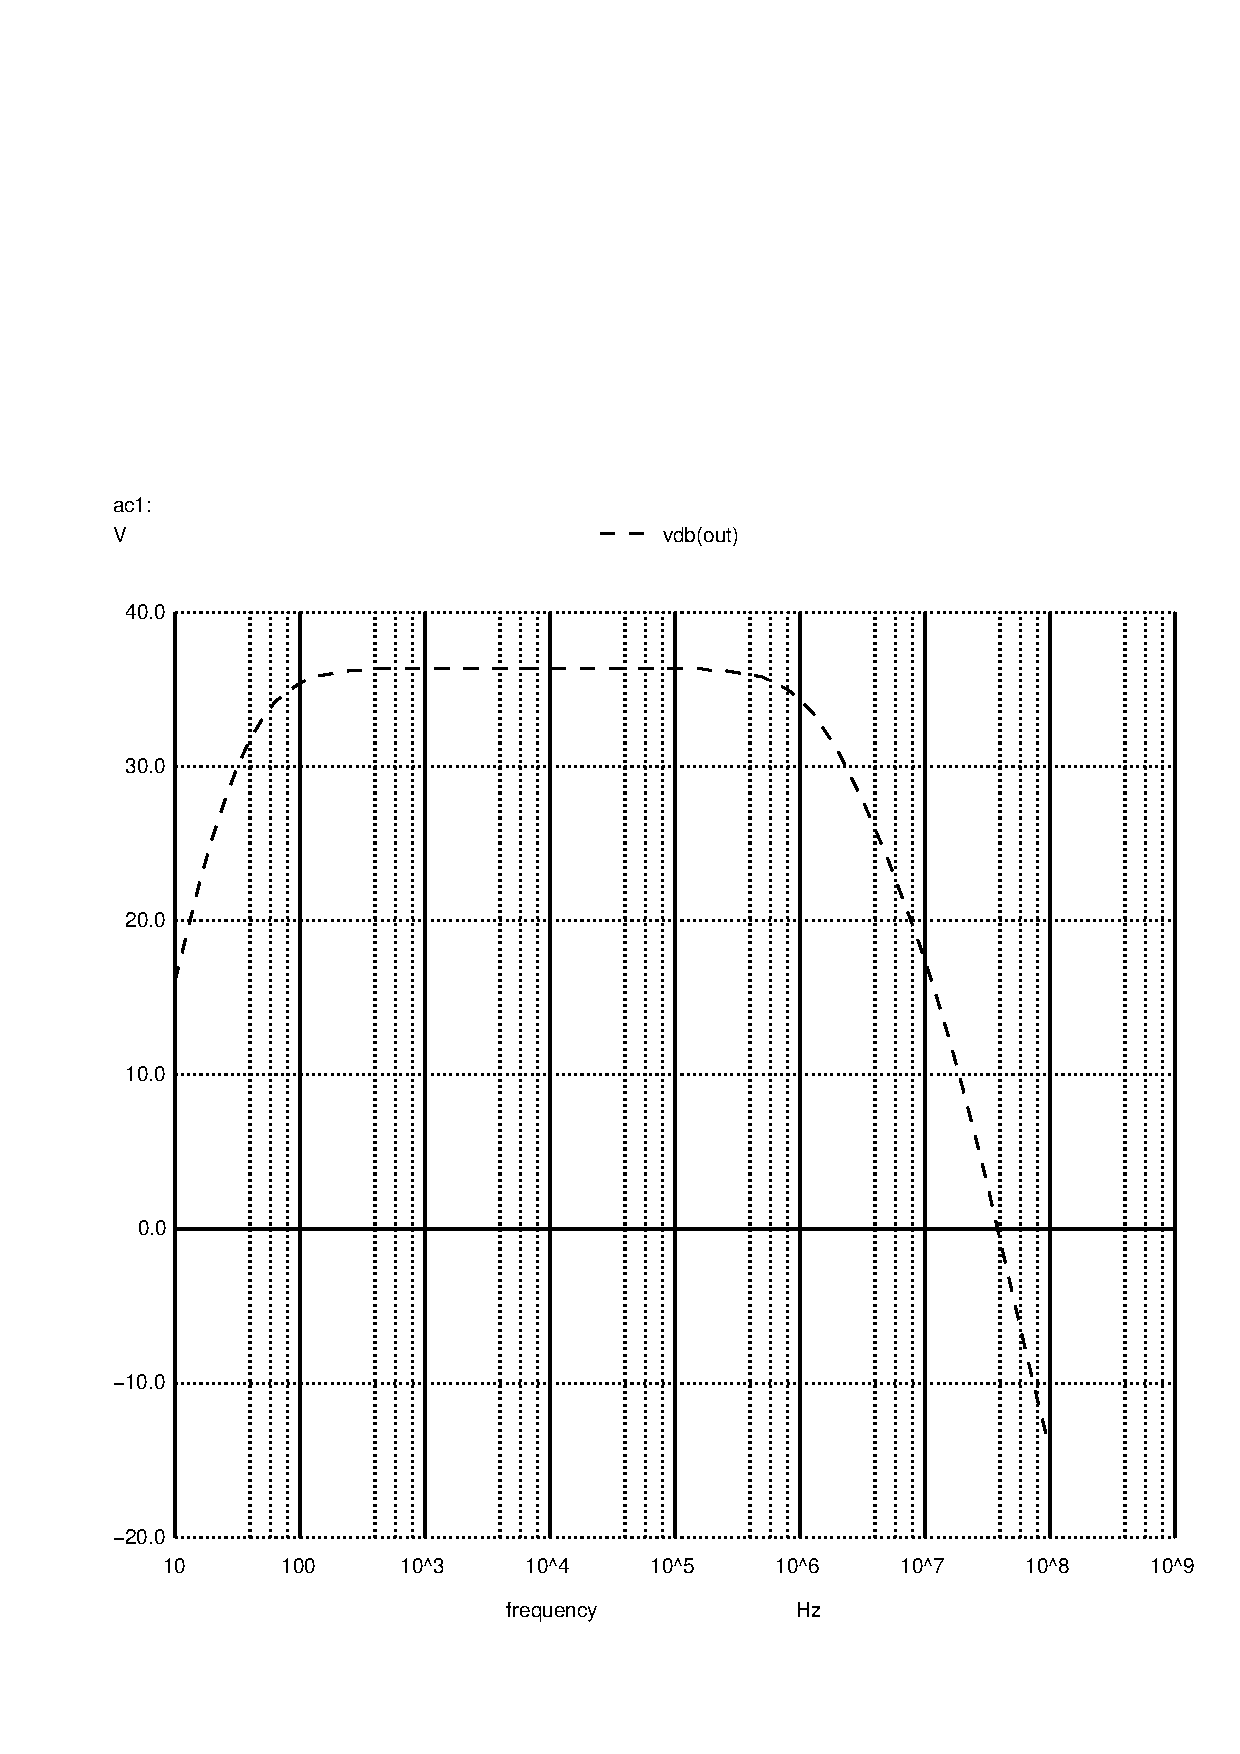
\includegraphics[width=0.4\linewidth]{vo2f.pdf}
\caption{Output voltage}
\label{fig:sim5}
\end{figure}




\item Determination of the imput impedance, seen from the imput voltage source.

\begin{table}[h]
  \centering
  \begin{tabular}{|l|r|}
    \hline    
   Zin & 999.002 + -7.3282 j\\ \hline

   \end{tabular}
  \caption{Input impedance in Ohm}
    \label{tab:ZI}
\end{table}

\par The result obtained for the imput impedance, considering the value in Kohm, is high. This is benefitial for the gain, because the voltage in the node In 2 must be as similiar to Vin as possible. Using a voltage dividir, the only way to achieve this was to have a very high resistance value.

\item Determination of the output impedance, using a different set up, seen from the load resistance. 

\begin{table}[h]
  \centering
  \begin{tabular}{|l|r|}
    \hline    
   Zo & 0.0522978 + -7.23396 j\\ \hline

   \end{tabular}
  \caption{Output impedance in Ohm}
  
  \label{tab:ZO}
\end{table}


Conserning the output impedance, an opposite deduction to the one made for the output impedance is mandoratory. Considering a voltage divider, the output impedance must be as low as possible, in order to the output voltage to be as high as possible. Having said that, an analysing tables \ref{tab:ZI} \ref{tab:ZO}, the difference needed between the two is confirmed. The output impedance obtained is favorable to the 8 ohm load resistance.

\item Compute of the cost and figure of merit
To finally understand the efficency of the amplifier, the cost and figure of merit were calculated

\begin{table}[ht]
  \centering
  \begin{tabular}{|l|r|}
    \hline    
   Cost & 1225.6\\ \hline
merit & 716.238\\ \hline

   \end{tabular}
  \caption{Cost and Figure of merit}
  \label{tab:cost}
\end{table}

Analysing table \ref{tab:cost}, the results obtained may be considered satisfying.


\end{enumerate}



